\chapter {Implementation Plan}
\section{Gantt Chart}
\begin{figure}[H]
        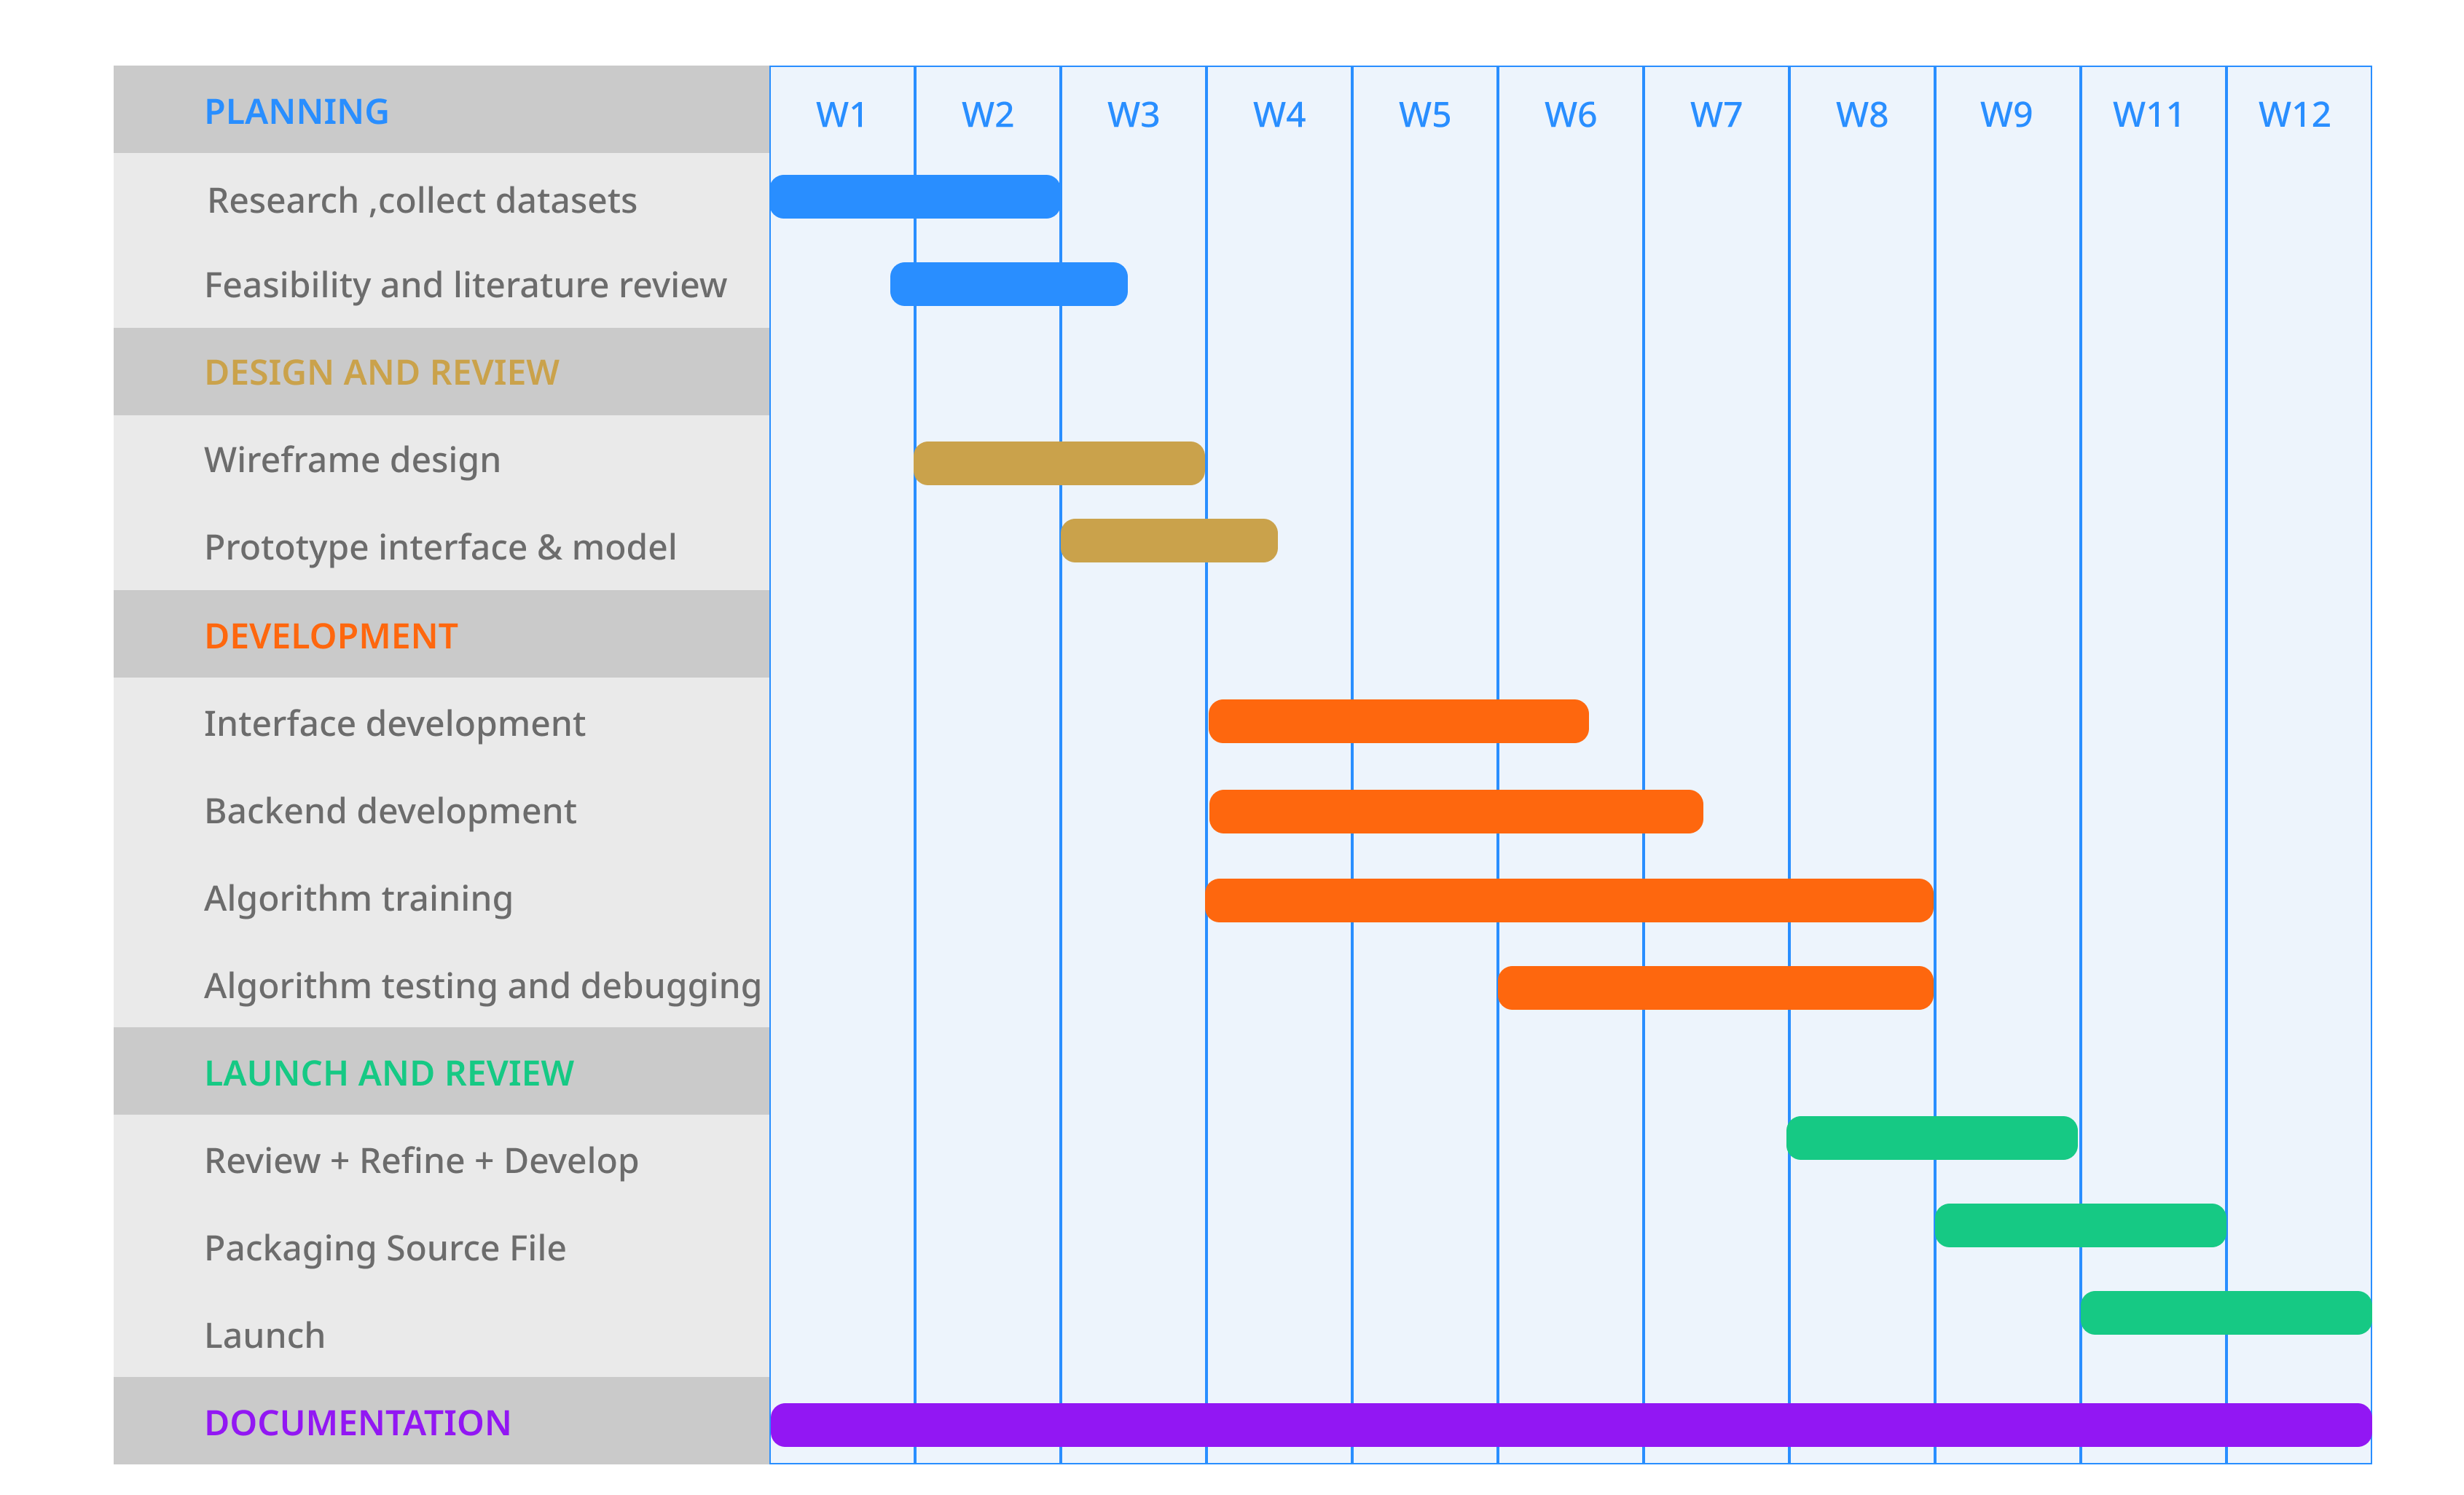
\includegraphics[width=150mm, left]{./img/gantt_chart.png}
\caption{Gantt Chart}
\end{figure}
\clearpage
\section{Software Requirement}
\begin{itemize}[noitemsep]
\item \textbf{Python:} 
Python is a versatile programming language commonly used for developing software applications. It can be used for various tasks in the system, such as backend development, data processing, and machine learning integration.
\item \textbf{MongoDB:}
MongoDB is a widely used NoSQL database, utilizes JSON-like documents for data storage, ensuring excellent performance and scalability. Its schema-less structure supports dynamic data modeling, making it well-suited for web applications. By employing collections instead of conventional tables and incorporating horizontal scaling, MongoDB efficiently handles diverse data types across multiple servers. This versatility positions it as a robust solution for contemporary, data-driven environments.
\item \textbf{React }
 React is a JavaScript library for building user interfaces, particularly in single-page applications. Developed by Facebook, it uses a declarative approach for efficiently updating the DOM. With a component-based structure, React enhances modularity and reusability, making it a popular choice for creating interactive and scalable web applications.
\item \textbf{Javascript:}
JavaScript is a programming language commonly used for developing web-based applications. It can be used for front-end development, implementing interactive features on the system’s web interface, and facilitating communication with the backend. 
\item \textbf{GitHub:}
GitHub is a web-based platform for version control using Git. It provides a collaborative environment for software development projects, allowing developers to host and share their code, track changes, manage workflows, and collaborate with others. GitHub offers features such as code repositories, issue tracking, project management tools, code review, and continuous integration.
\item \textbf{MATLAB:}
MATLAB, short for ``Matrix Laboratory,'' is a high-level programming language and interactive environment primarily used for numerical computation, visualization, and programming. It provides a wide range of built-in functions and toolboxes for various applications, including mathematics, signal processing, image processing, control systems, and machine learning.
\item \textbf{VS Code:}
VS Code is a popular and widely used source code editor that offers a range of features and extensions to enhance the development experience. It supports multiple programming languages, including Python, JavaScript, and React, making it suitable for working with the different components of the system. 
\end{itemize}


\section{Hardware Requirement}
\begin{enumerate}[noitemsep] %label=\Roman*.]
   \item High dedicated RAM to handle memory-intensive tasks
   \item NVIDIA GPU for optimal performance.
   \item Dedicated GPU with CUDA support for accelerated parallel processing.
   \item  SSD storage for faster read/write speeds during image processing.
   \item Additional high-capacity external storage for storing large datasets and image collections.
   \item Smartphone or tablet for testing mobile applications  
\end{enumerate}
